\section{Results and Analysis}

In order to analyze the algorithms, we used both PAPI events and timed the algorithms for differently sized matrixes.
The data collected was saved in .csv files and transformed into graphics for better analysis.

\subsection{PAPI events inconsistencies}

At the beginning of the project we wanted to collect data about data cache accesses to calculate miss to access ratio.
As we analysed our data we found that most of the time data cache accesses were lower than misses. Later we found that PAPI gives no guaranties that data cache misses, accesses and hits have any correlation [1] so our analysis was limited do only data cache misses. We didn't used level 3 data cache accesses because this metric is the same as level 2 data cache misses as can be seen in PAPI event description. 

\subsection{Matrixes from 600x600 to 3000x3000}

\subsubsection{Execution time and \uppercase{FLOPS}}

When comparing the different algorithms that were implemented regarding execution times and \uppercase{GFLOPS} we can see that, as matrix size grows, \textbf{Multi-line Matrix Multiplication} is an order of magnitude more efficient than \textbf{Normal Matrix Multiplication}. 

The comparison between algorithms regarding GFLOPS shows that for the same matrixes, the computer performed more almost double the operations per second when running \textbf{Multi-line Matrix Multiplication} when compared with it's counterpart. This indicates that \textbf{Multi-line Matrix Multiplication} is using the computer resources more efficiently as we will discuss below.

The tendencies described above were verified both on C++ and Java. Java being a high-level language performed worse than C++ in \textbf{Normal Matrix Multiplication}. This tendency was not verified in \textbf{Multi-line Matrix Multiplication} for this matrix sizes with Java performing as good as C++. This can be explained because the algorithm is more efficient so performance trade-offs were not observed.

\begin{figure}[H]
    \begin{minipage}{.5\textwidth}
        \centering
        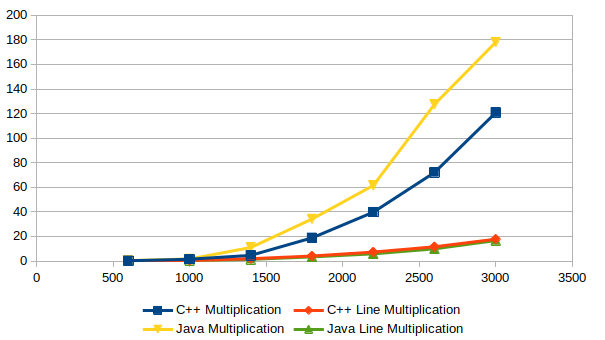
\includegraphics[width=\linewidth]{img/small_execution_time.png}
        \captionof{figure}{Execution Time (s)}
        \label{fig:test1}
    \end{minipage}
    \begin{minipage}{.5\textwidth}
        \centering
        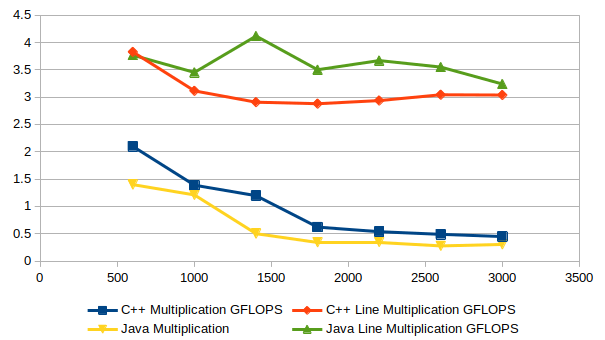
\includegraphics[width=\linewidth]{img/small_flops.png}
        \captionof{figure}{Float Operations (\uppercase{GFLOPS})}
        \label{fig:test1}
    \end{minipage}%
\end{figure}

\subsubsection{PAPI events analysis}

The comparison of the \textbf{data cache misses} in L1 and L2 (PAPI\_L1\_DCM and PAPI\_L2\_DCM) between \textbf{Normal Matrix Multiplication} and \textbf{Multi-line Matrix Multiplication} draws us corroborate our theories: the second method of matrix multiplication avoids many cache misses. Although we expected to see a higher number of L1 cache misses than L2 cache misses, because there is some data that might not be present in L1 cache but might be in L2 cache, our data contradicts this fact.

\begin{figure}[H]
    \centering
    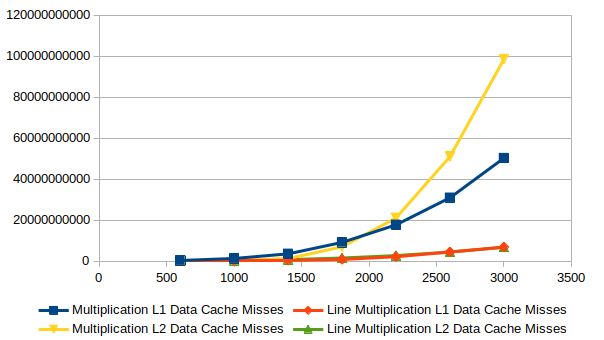
\includegraphics[width=.8\linewidth]{img/small_cache.png}
    \caption{Number of cache misses related to matrix size}
\end{figure}

\subsection{Matrixes from 4098x4098 to 10240x10240}

\subsubsection{Execution time and \uppercase{FLOPS}}

The comparison between \textbf{Multi-line Matrix Multiplication} and \textbf{Block Matrix Multiplication} in terms of execution time reveals that the second algorithm is more efficient independently of matrix and block size. Between different block sizes we observed that the execution time decreases when comparing 128x128 with 256x256 matrixes, and then it starts increasing again. We can conclude that 256x256 blocks seem to be the ideal size of block for this configuration. The analysis of \uppercase{FLOPS} proved that \textbf{Block Matrix Multiplication} with a block size of 256x256 yielded the best result.

\begin{table}[H]
\centering
\begin{tabular}{ll|lllll|}
\cline{3-7}
\multicolumn{2}{l|}{\multirow{2}{*}{}} & \multicolumn{5}{c|}{Algorithm} \\ \cline{3-7} 
\multicolumn{2}{l|}{} & \multicolumn{1}{l|}{\begin{tabular}[c]{@{}l@{}}Line\\ Multiplication\end{tabular}} & \multicolumn{1}{l|}{\begin{tabular}[c]{@{}l@{}}Block\\ Multiplication \\ (128)\end{tabular}} & \multicolumn{1}{l|}{\begin{tabular}[c]{@{}l@{}}Block\\ Multiplication \\ (256)\end{tabular}} & \multicolumn{1}{l|}{\begin{tabular}[c]{@{}l@{}}Block\\ Multiplication \\ (512)\end{tabular}} & \begin{tabular}[c]{@{}l@{}}Block\\ Multiplication \\ (1024)\end{tabular} \\ \hline
\multicolumn{1}{|l|}{\multirow{4}{*}{\rotatebox[origin=c]{90}{Matrix Size}}} & 4096 & \multicolumn{1}{l|}{49.3273} & \multicolumn{1}{l|}{39.7087} & \multicolumn{1}{l|}{36.7971} & \multicolumn{1}{l|}{46.8632} & 40.9488 \\ \cline{2-7} 
\multicolumn{1}{|l|}{} & 6144 & \multicolumn{1}{l|}{162.744} & \multicolumn{1}{l|}{134.351} & \multicolumn{1}{l|}{122.605} & \multicolumn{1}{l|}{127.923} & 139.881 \\ \cline{2-7} 
\multicolumn{1}{|l|}{} & 8192 & \multicolumn{1}{l|}{414.092} & \multicolumn{1}{l|}{345.589} & \multicolumn{1}{l|}{370.028} & \multicolumn{1}{l|}{389.386} & 342.124 \\ \cline{2-7} 
\multicolumn{1}{|l|}{} & 10240 & \multicolumn{1}{l|}{763.512} & \multicolumn{1}{l|}{635.891} & \multicolumn{1}{l|}{578.957} & \multicolumn{1}{l|}{612.065} & 679.643 \\ \hline
\end{tabular}
\caption{Execution Time (s)}
\end{table}

\begin{figure}[H]
    \centering
    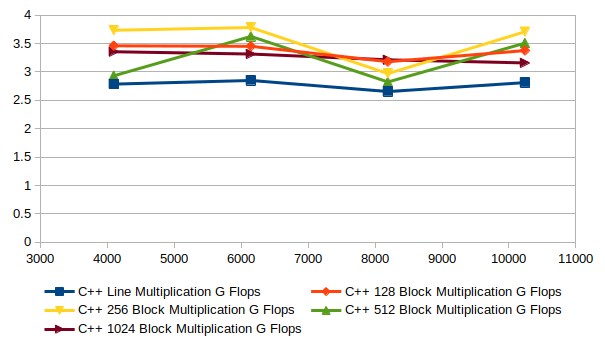
\includegraphics[width=.8\linewidth]{img/big_flops.png}
    \caption{Float Operations (\uppercase{GFLOPS})}
\end{figure}

\subsubsection{PAPI events analysis}

As we observed with smaller matrix sizes the number of cache L2 cache misses is greater than the number of L1 cache misses. The number of cache misses in both level one and level two caches in \textbf{Multi-line Matrix Multiplication} is the double of \textbf{Block Matrix Multiplication} this justifies why \textbf{Multi-line Matrix Multiplication} is much slower than \textbf{Block Matrix Multiplication}. Between different block sizes we observed that the number of cache misses in both level of caches is decresing as the size of the block increases. This fact does not explain why execution time increases as block size increases.

\begin{table}[H]
\centering
\begin{tabular}{ll|lllll|}
\cline{3-7}
\multicolumn{2}{l|}{\multirow{2}{*}{}} & \multicolumn{5}{c|}{Algorithm} \\ \cline{3-7} 
\multicolumn{2}{l|}{} & \multicolumn{1}{l|}{\begin{tabular}[c]{@{}l@{}}Line\\ Multiplication\end{tabular}} & \multicolumn{1}{l|}{\begin{tabular}[c]{@{}l@{}}Block\\ Multiplication \\ (128)\end{tabular}} & \multicolumn{1}{l|}{\begin{tabular}[c]{@{}l@{}}Block\\ Multiplication \\ (256)\end{tabular}} & \multicolumn{1}{l|}{\begin{tabular}[c]{@{}l@{}}Block\\ Multiplication \\ (512)\end{tabular}} & \begin{tabular}[c]{@{}l@{}}Block\\ Multiplication \\ (1024)\end{tabular} \\ \hline
\multicolumn{1}{|l|}{\multirow{4}{*}{\rotatebox[origin=c]{90}{Matrix Size}}} & 4096 & \multicolumn{1}{l|}{17.647795712} & \multicolumn{1}{l|}{9.613625662} & \multicolumn{1}{l|}{9.053586218} & \multicolumn{1}{l|}{8.766963868} & 8.785341456 \\ \cline{2-7} 
\multicolumn{1}{|l|}{} & 6144 & \multicolumn{1}{l|}{59.561360444} & \multicolumn{1}{l|}{32.437636037} & \multicolumn{1}{l|}{30.540354075} & \multicolumn{1}{l|}{29.638354628} & 29.690638422 \\ \cline{2-7} 
\multicolumn{1}{|l|}{} & 8192 & \multicolumn{1}{l|}{141.119280713} & \multicolumn{1}{l|}{76.943793304} & \multicolumn{1}{l|}{72.472340236} & \multicolumn{1}{l|}{70.217429601} & 70.384445555 \\ \cline{2-7} 
\multicolumn{1}{|l|}{} & 10240 & \multicolumn{1}{l|}{275.441489151} & \multicolumn{1}{l|}{150.101146037} & \multicolumn{1}{l|}{141.423714683} & \multicolumn{1}{l|}{137.100929723} & 137.52190264 \\ \hline
\end{tabular}
\caption{L1 Cache Misses (Miss×10^{9})}
\end{table}

\begin{table}[H]
\centering
\begin{tabular}{ll|lllll|}
\cline{3-7}
\multicolumn{2}{l|}{\multirow{2}{*}{}} & \multicolumn{5}{c|}{Algorithm} \\ \cline{3-7} 
\multicolumn{2}{l|}{} & \multicolumn{1}{l|}{\begin{tabular}[c]{@{}l@{}}Line\\ Multiplication\end{tabular}} & \multicolumn{1}{l|}{\begin{tabular}[c]{@{}l@{}}Block\\ Multiplication \\ (128)\end{tabular}} & \multicolumn{1}{l|}{\begin{tabular}[c]{@{}l@{}}Block\\ Multiplication \\ (256)\end{tabular}} & \multicolumn{1}{l|}{\begin{tabular}[c]{@{}l@{}}Block\\ Multiplication \\ (512)\end{tabular}} & \begin{tabular}[c]{@{}l@{}}Block\\ Multiplication \\ (1024)\end{tabular} \\ \hline
\multicolumn{1}{|l|}{\multirow{4}{*}{Matrix Size}} & 4096 & \multicolumn{1}{l|}{17.209304763} & \multicolumn{1}{l|}{30.272506811} & \multicolumn{1}{l|}{22.718508038} & \multicolumn{1}{l|}{19.089596015} & 18.635256131 \\ \cline{2-7} 
\multicolumn{1}{|l|}{} & 6144 & \multicolumn{1}{l|}{57.841281211} & \multicolumn{1}{l|}{107.174007311} & \multicolumn{1}{l|}{30.540354075} & \multicolumn{1}{l|}{64.757090769} & 64.494440561 \\ \cline{2-7} 
\multicolumn{1}{|l|}{} & 8192 & \multicolumn{1}{l|}{136.827183508} & \multicolumn{1}{l|}{247.599027107} & \multicolumn{1}{l|}{177.171570622} & \multicolumn{1}{l|}{150.843420658} & 150.278383529 \\ \cline{2-7} 
\multicolumn{1}{|l|}{} & 10240 & \multicolumn{1}{l|}{289.717224388} & \multicolumn{1}{l|}{495.942550318} & \multicolumn{1}{l|}{356.950322647} & \multicolumn{1}{l|}{305.120720325} & 292.778686636 \\ \hline
\end{tabular}
\caption{L2 Cache Misses (Miss×10^{9})}
\end{table}
